\section{Dockerにおけるビルドの失敗に関する調査\cite{docker-failures}}
\subsection{概要}
Dockerは近年,コンテナ型仮想化技術の世界標準として注目を浴びている.しかし,Dockerのビルドは頻繁に失敗し,その修正には長い時間を要することが度々ある.これまでの研究では,大規模開発でのDockerのビルド失敗率について調査した研究はあったが,失敗の頻度とその修正に関する調査を行った研究はほとんど存在していなかった.文献\cite{docker-failures}では,Githubにリンクされた3,828件のオープンソースプロジェクトの857,086件のDockerのビルドについて調査している.Dockerのビルドデータを用いて,以下の3つのRQについて調査を行っている.

\begin{itemize}
  \item RQ 1: Dockerのビルドはどれくらいの頻度で失敗するか?
  \item RQ 2: ビルドの修正を行うのにどれくらいの時間を要するか?
  \item RQ 3: ビルド失敗の頻度と修正時間は時間の経過によってどのような関係性があるか?
\end{itemize}

% ====== 結果いるのかな? ==========
% その結果,

\subsection{データ収集}
ここではデータの収集について説明する.文献\cite{docker-failures}では,公開されているDockerプロジェクトのビルドデータを取得するため,DockerHub APIで ``is\_autoomated"という文字列の有無をチェックして公開されているプロジェクトの特定を行っている.特定したプロジェクトからビルド数が10以下のプロジェクトをフィルタリングして,最終的に3,828件のプロジェクトのデータセット,857,086件のDockerビルドデータ(メタデータを含む)を取得している.表\ref{fig:3_docker-build-data}に各プロジェクトにおけるビルド数の統計値を示す.


\begin{table}[t]
    \centering
    \caption{各プロジェクトにおけるビルド数の基本統計}
    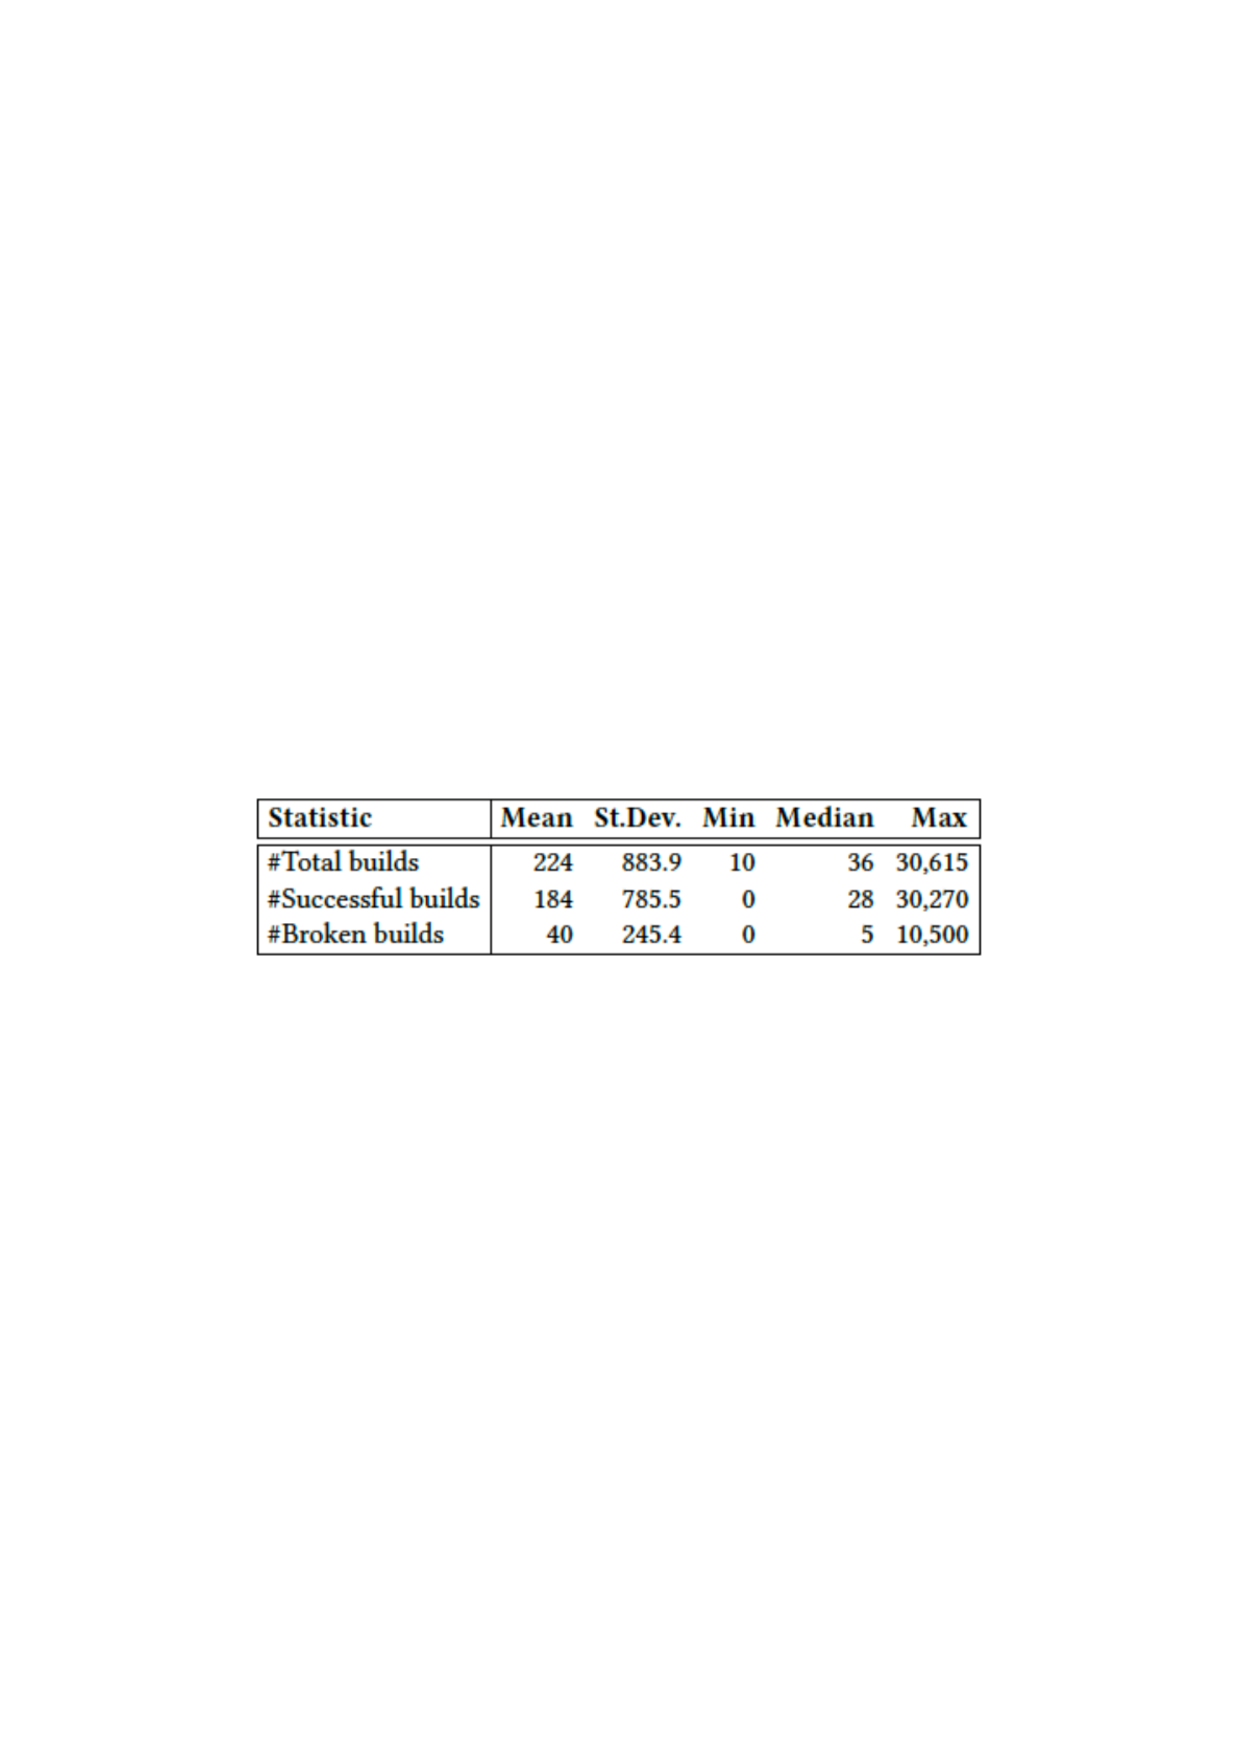
\includegraphics[width=0.9\linewidth, angle=0]{./thesis3/docker-build-data3.pdf}
    \label{fig:3_docker-build-data}
\end{table}

\subsection{データ処理}

\begin{figure}[t]
    \centering
    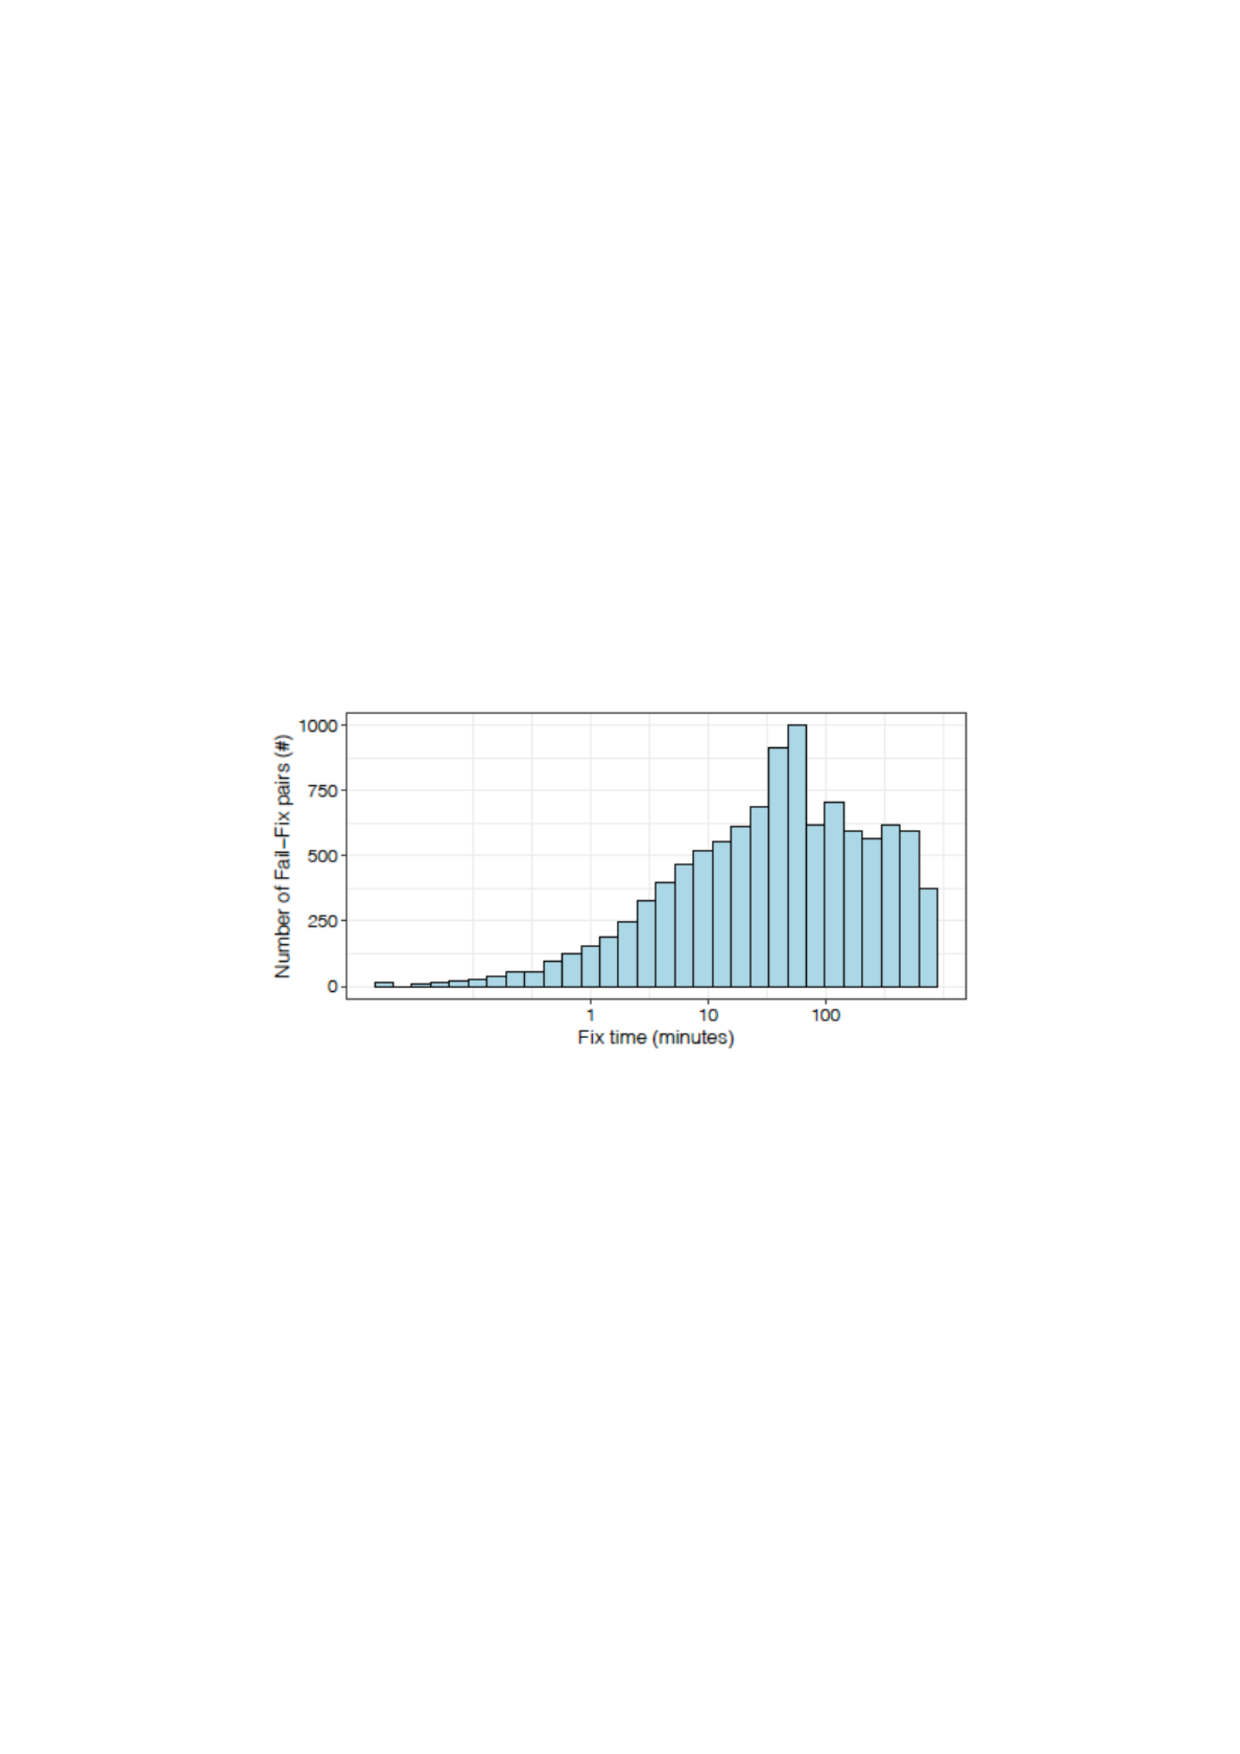
\includegraphics[width=0.9\linewidth, angle=0]{./thesis3/docker-build-failuer-number3.pdf}
    \caption{修正時間の分布}
    \label{fig:3_docker-build-failuer-number}
\end{figure}

\begin{figure}[t]
    \centering
    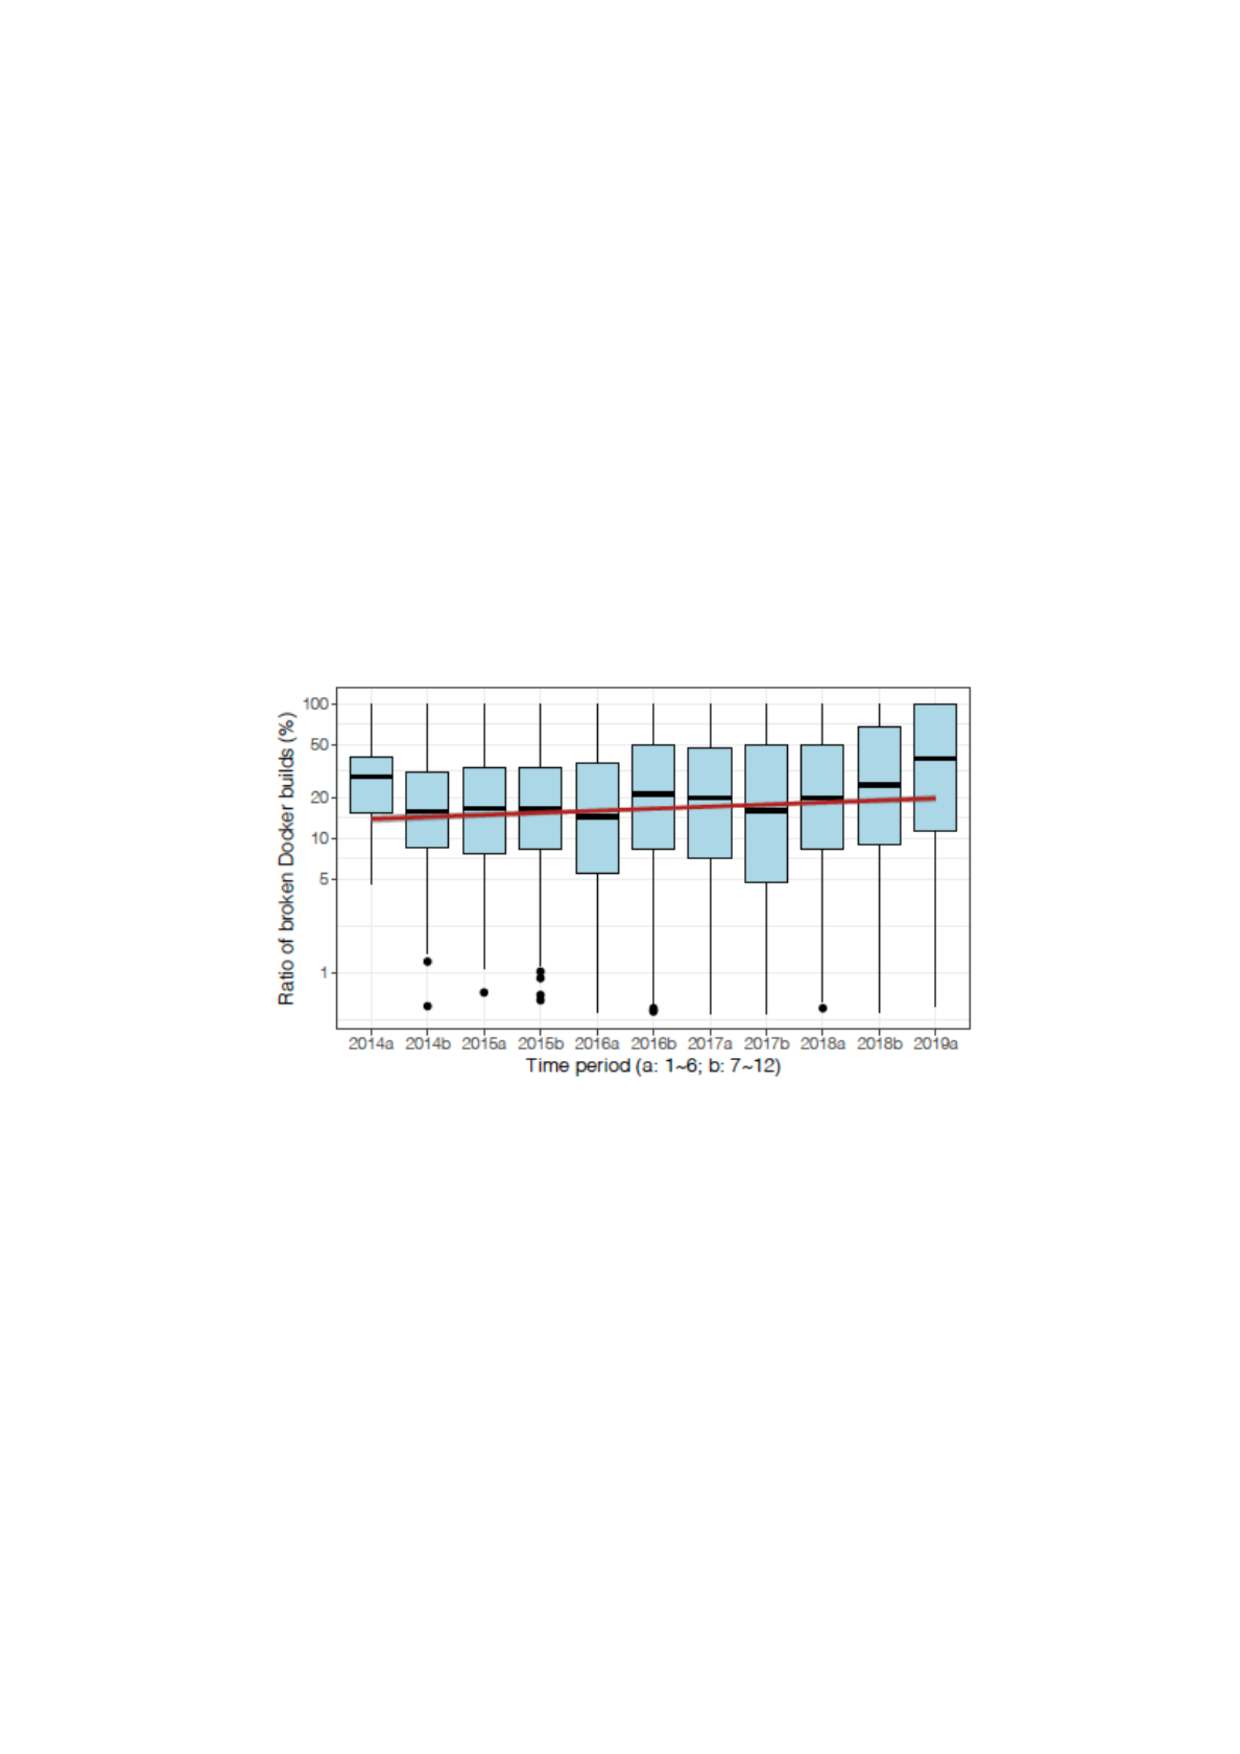
\includegraphics[width=0.9\linewidth, angle=0]{./thesis3/docker-build-failuer-ratio-period3.pdf}
    \caption{6ヶ月間のビルドの失敗率の分布}
    \label{fig:3_docker-build-failer-ratio-period}
\end{figure}

\begin{figure}[t]
    \centering
    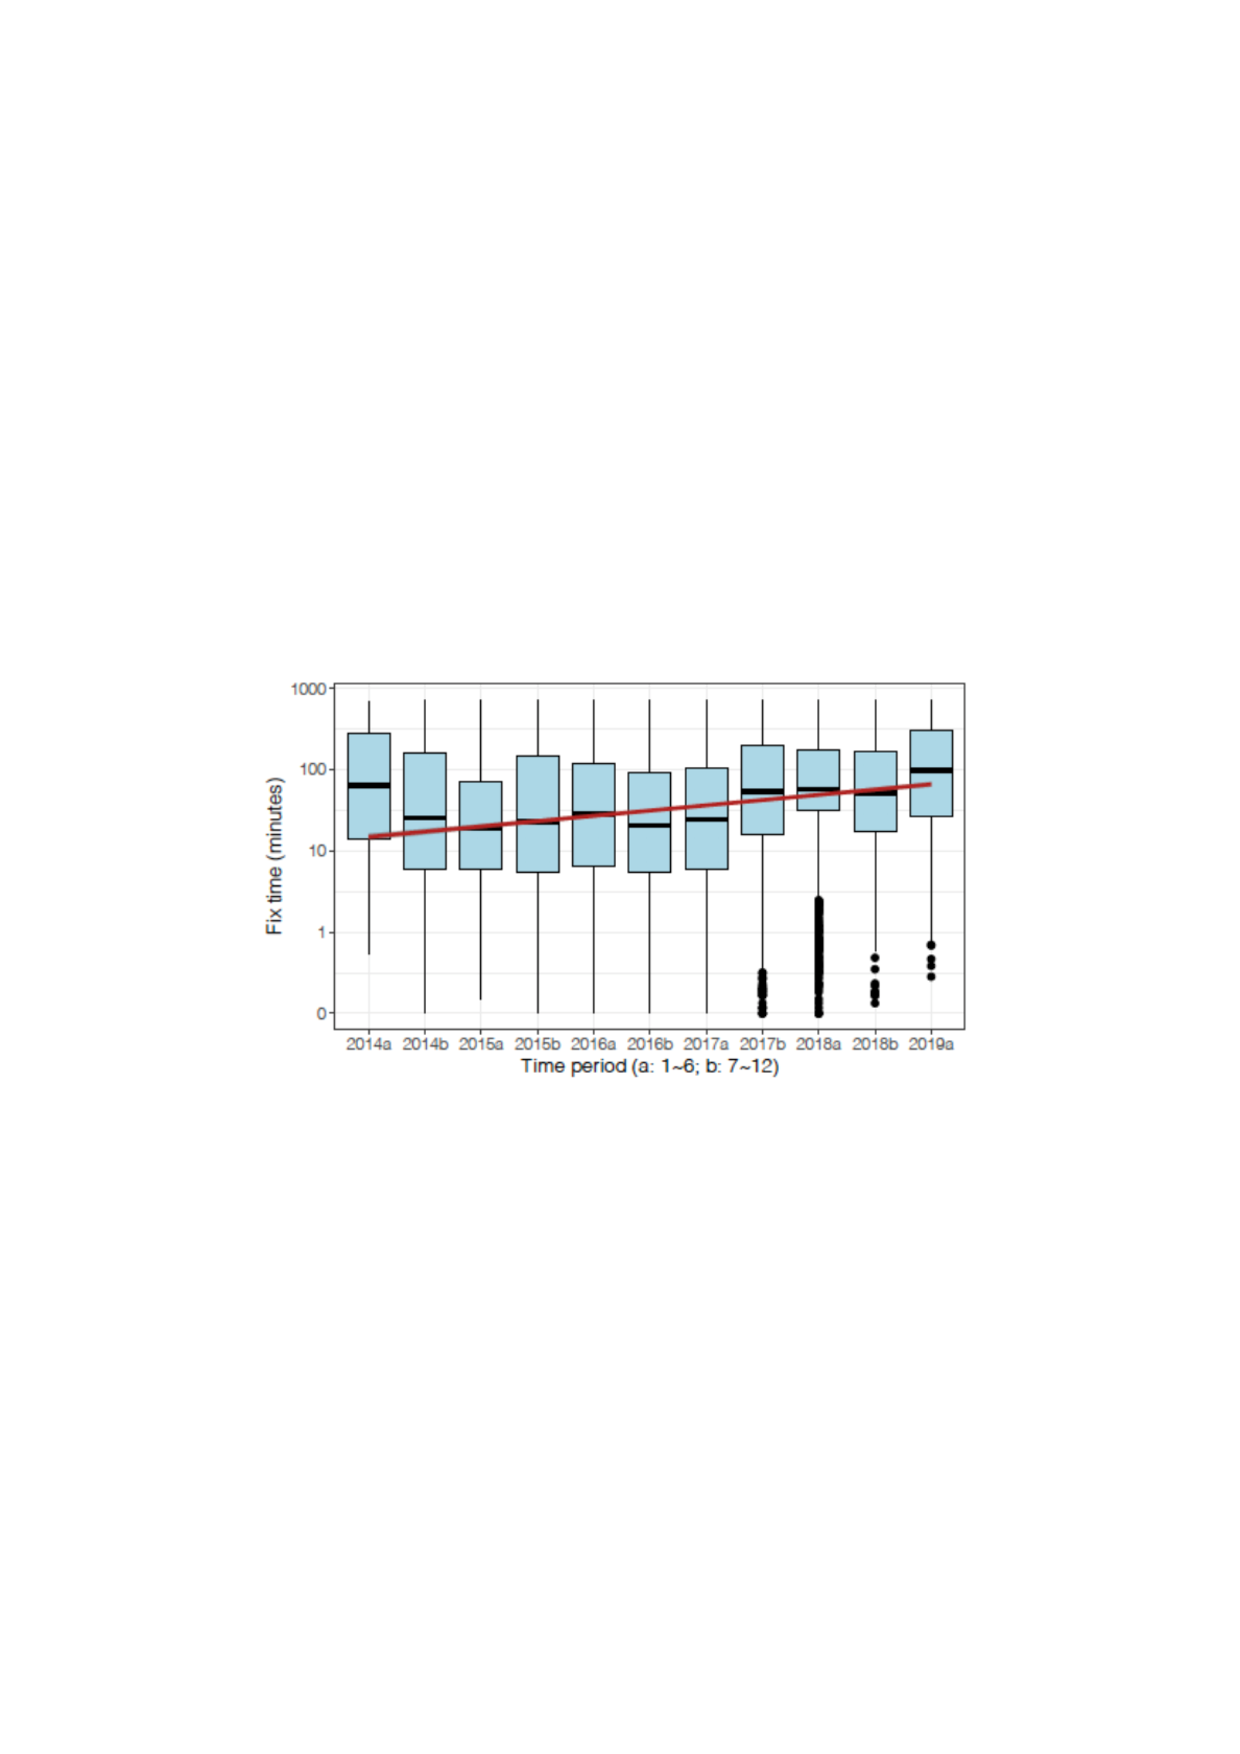
\includegraphics[width=0.9\linewidth, angle=0]{./thesis3/docker-build-fix-time-period3.pdf}
    \caption{6ヶ月間の修正時間の分布}
    \label{fig:3_docker-build-fix-time-period}
\end{figure}

RQ2についてビルドの修正時間にどれくらいの時間を要するかを分析するために,バグとその修正のペアの特定を行っている.

% 文献\cite{docker-failures}ではRabbaniら\cite{3-ref-5}が提案したバグとその修正のペアを特定する方法を用いている.

具体的には,ビルドが成功した直後に続く失敗したビルド(A)を発見し,次に発見する成功したビルド(B)のABのペアを,ビルドの失敗とその修正としている.ここで開発者のスケジュールが修正時間に影響しないように,修正時間が12時間を超えるものをフィルタリングしている.図\ref{fig:3_docker-build-failuer-number}にDockerビルドの修正時間の分布を示す.

% === RQ2の考察 =======
% 有効な10,566件のFail-Fixペアのうち、511件(4.8%)が1分未満、2,105件(19.9%)が1分から10分、4,511件(42.7%)が10分から100分、3,431件(32.5%)が100分以上の時間を要しています。
% 我々のデータセットでは、壊れたビルドの修正に平均124.5分(中央値:44.2分)かかり、これはGoogleの研究(12分未満)よりもはるかに長いです[7]。
% この差には、作業環境やツールなど多くの要因が関係していると考えられる。また、この差が大きいのは、Google が開発者の広範囲に影響を与えないように、開発者に障害発生時の迅速な対応を要求しているためと考えられる[11]。しかし、オープンソースプロジェクトの開発者がこのような規制を完全に遵守することは困難です。また、従来のビルドプロセスとは異なり、各Dockerビルドは、コードからパッケージング、テスト、クラウドレジストリへのプッシュまでのプロセスを完了させる必要があり、長い時間がかかる可能性があります。
% このため、開発者は最終的なビルド結果を見て不具合が修正されたかどうかを判断するために長い時間を待つことになり、Dockerビルドの不具合修正にマイナスの影響を与える可能性があります。そのため、開発者に潜在的なビルド結果(例えば、失敗か成功か、ビルドが失敗した場合の修正時間の予測など)を思い出させるためのビルド予測技術が必要とされています。
% % その結果、プロジェクトあたりの壊れたビルド数は、修正時間の中央値と正の相関があることがわかりました(スピアマンのrho=0.28、p<0.001)。このように、ビルド数が多いプロジェクトほど、修正時間が長くなることがわかりました。失敗が多すぎると、開発者の時間と集中力が散漫になり、その結果、困難な失敗や重要な失敗を時間内に修正することができないことがある。

また,RQ3についてDockerのビルドの失敗とその修正時間の,時間経過による関係性を調査するため,6ヶ月間の期間ごとにデータを集計する.その結果を図\ref{fig:3_docker-build-failer-ratio-period},図\ref{fig:3_docker-build-fix-time-period}に示す.



% \begin{figure}[t]
%     \centering
%     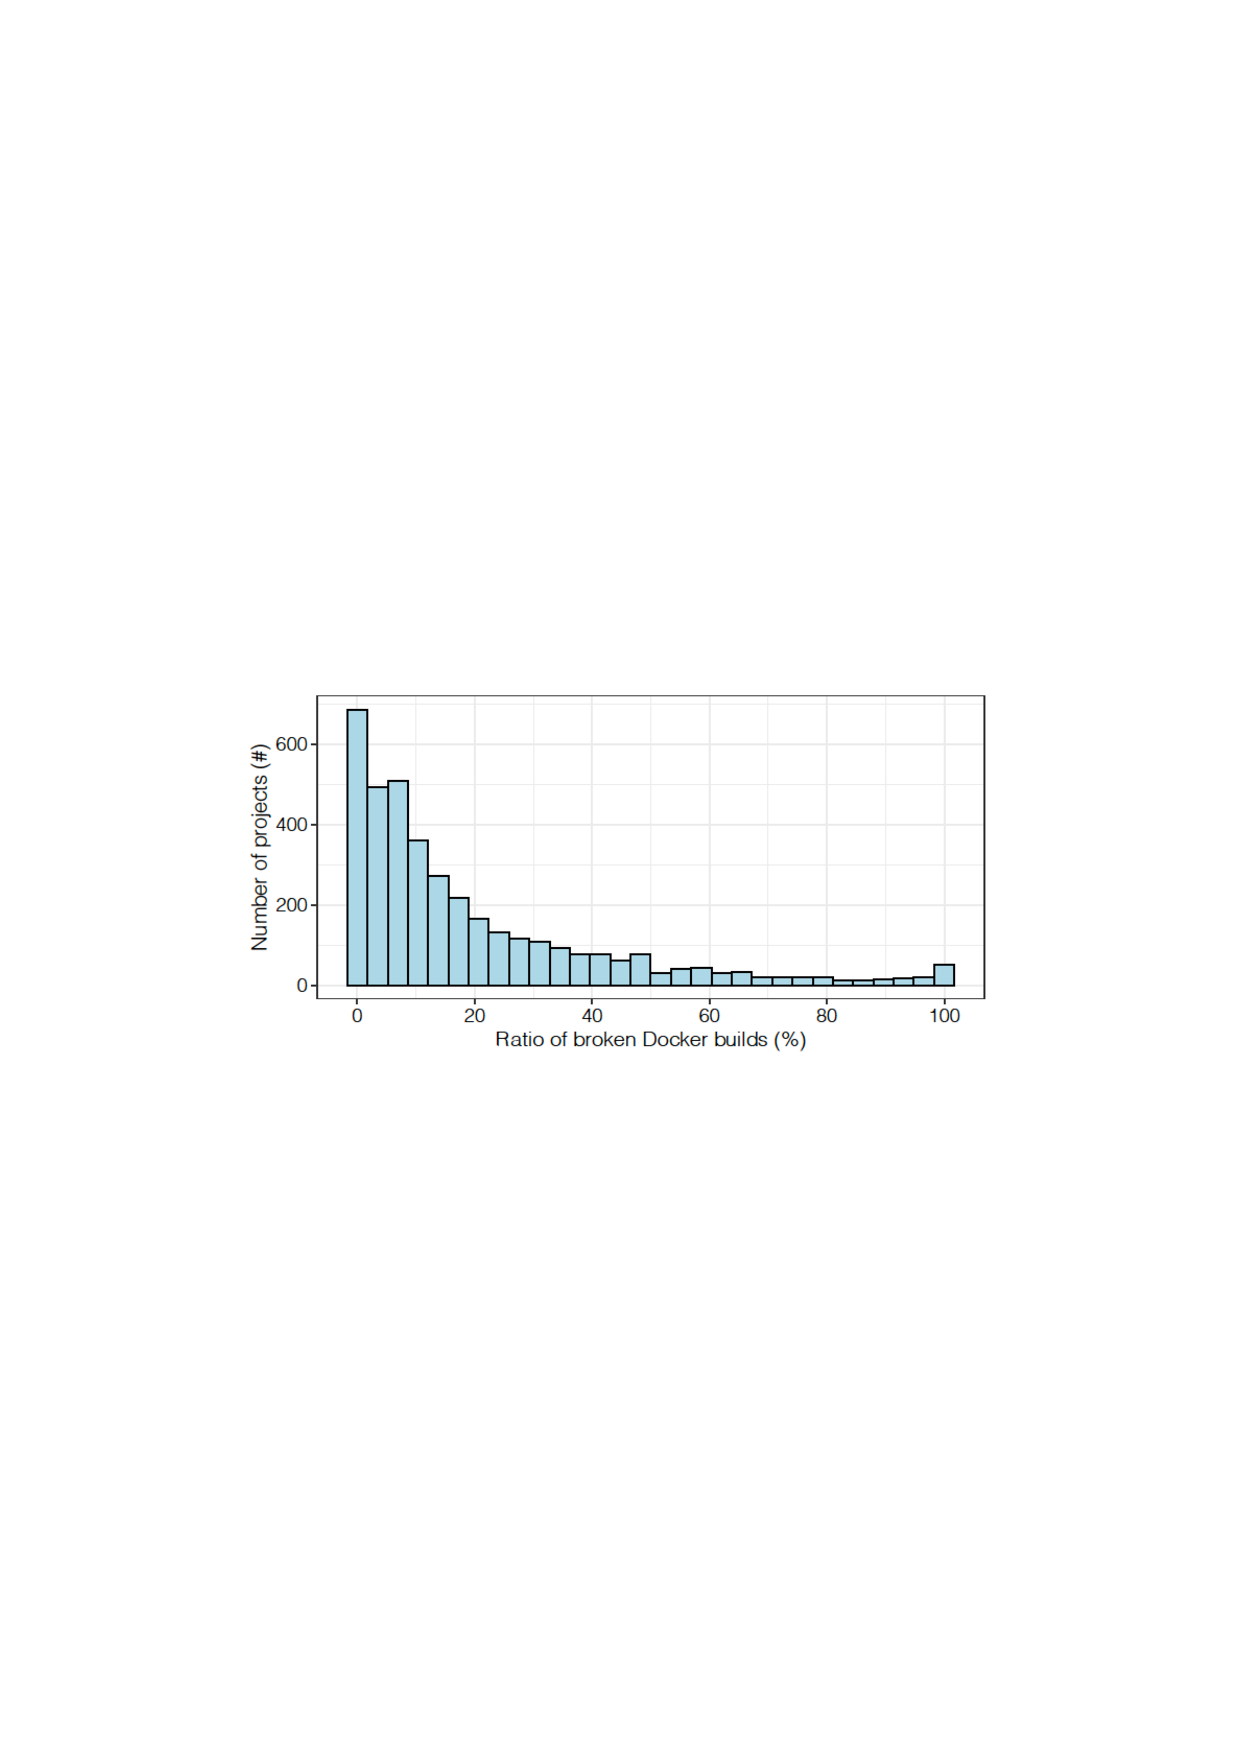
\includegraphics[width=0.9\linewidth, angle=0]{./thesis3/docker-build-number3.pdf}
%     \label{fig:3_docker-build-number}
%     \caption{ビルド失敗件数の分布}
% \end{figure}


\subsection{結果}
文献\cite{docker-failures}では,Docker環境におけるビルドの失敗事例について,大規模な実証実験を行っている.その結果,対象にした3,828件のプロジェクトにおいて,85.2\%のプロジェクトでビルドが発生しており,857,086件のビルドデータのうち17.8\%が失敗しているということが明らかになっている.また,31.5\%のプロジェクトにおいて,ビルドの20\%以上が失敗している.
% しかし,頻繁にビルドされているプロジェクトでは,ビルド失敗の割合は比較的低くなっている
失敗したビルドの修正時間については,平均124.5分,中央値が44.2分であり,ビルドの失敗が頻繁に発生するプロジェクトでは,その修正時間が長いという結果も示されている.この結果は従来のビルドプロセスよりも長い時間になっている.
文献\cite{docker-failures}では,Dockerのビルドは従来と異なりコードからパッケージング,テスト,クラウドへのデプロイまでのプロセスがあり,修正に長い時間がかかるために,ビルドの失敗が多いほど修正時間も長くなっていくと示唆している.
また,図\ref{fig:3_docker-build-failer-ratio-period},図\ref{fig:3_docker-build-fix-time-period}よりDockerのビルドが失敗する割合やその修正に要する時間は,時間の経過とともにどちらも増加する傾向があるということが示されている.

% 先行研究\cite{3-ref-12}では,Dockerのビルドにかかる遅延時間が時間の経過とともに増加する傾向があることが確認されている.時間,負荷のかかるビルドは,失敗率を高める可能性があり,さらにRQ2で示されたように,より多くのビルドの失敗数と修正時間には相関があることが示されている.文献\cite{docker-failures}ではこれらの要因により,ビルド失敗率と修正時間が時間の経過とともに増加する可能性があると示唆している.

文献\cite{docker-failures}より,Dockerにおいてビルドの失敗とその修正時間は時間の経過とともに長くなっていくことがわかり,その原因としてDockerにおける開発手法の知見が不足していることが考えられる.また同時に,Dockerfile内にビルドの失敗に関係するようなSATDコメントが含まれることが考えられ,SATDの返済について調査を行うことは,Dockerにおけるビルドの失敗や潜在するバグの問題を解決するのに有効であると考えられる.